\begin{frame}{And now for something completely different...}
	\begin{center}
		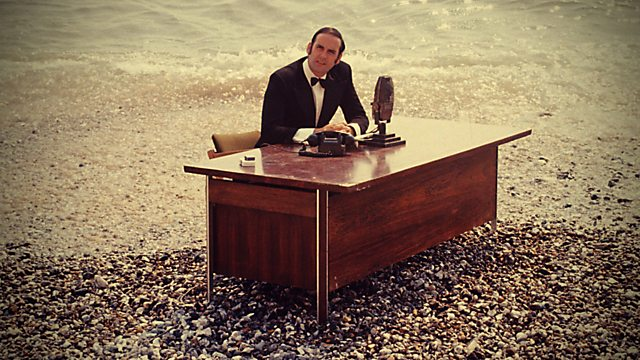
\includegraphics[width=\textwidth]{figures/something_different.jpg}
	\end{center}
	We would like to define \textbf{sheaves on arbitrary categories}: in fact, there are presheaves on any category, why shouldn't we have sheaves?
\end{frame}

\begin{frame}{The topos of presheaves}
	Now $\Set^{\cat C^\op}$ inherits a lot of good structure from $\Set$:
	\begin{enumerate}
		\item<2-> Completeness (pointwise limits) and cocompleteness (formal colimits)
		\item<3-> Exponentials:
		\begin{equation*}
			G^F(U) \iso \Nat(\yo U, G^F) \iso \Nat(\yo U \times F, G)
		\end{equation*}
		\item<4-> Subobject classifier: $\Omega(U) =$ subfunctors of $\yo U$ = $\Sub(\yo U)$.
		\begin{diagram*}
			P \arrow[tail, swap]{d}{\forall \varphi} \arrow{r}{!} \& 1 \arrow{d}{\true} \&[-3ex] \color{colornote}{*} \arrow[colornote, mapsto]{d}\\
			F \arrow{r}{\exists ! \ulcorner \varphi \urcorner} \& \Omega \& \color{colornote}{1_{\yo U}}
		\end{diagram*}
	\end{enumerate}
	\onslide<5->{
		A category satisfying these properties is called a \defining{Grothendieck topos}. If it's only \emph{finitely} bicomplete, it's an \defining{elementary topos}.
	}
\end{frame}

\begin{frame}{Internal language of topoi}
	An elementary topos has a rich internal language

	description
	$\Omega$ object of `truth values' or `propositions'
\end{frame}

\begin{frame}{Internal language of topoi}
	The internal language can simplify dealing with presheaves by transforming complex sheaf-theoretical theorems/proofs/constructions into easy set-theoretical theorems/proofs/constructions.
	\begin{diagram*}
		 classic twisted arrow diagram
	\end{diagram*}
\end{frame}

\begin{frame}{Lawvere--Tierney topologies}
	The internal language can also be used to describe sheaves!
	\begin{definition}
		Lawvere--Tierney topology
	\end{definition}
	The modality expressed by an LT topology is the `locally' modality.
	\begin{definition}
		A sheaf is a modal type for (the monad induced by) a Lawvere--Tierney topology
	\end{definition}
	Indeed: \textbf{a sheaf is `something defined locally'}.
\end{frame}

\begin{frame}{Lawvere--Tierney topologies}
	How does this fit into the `sheaf as continuous functors' perspective?
\end{frame}

\begin{frame}{Sites}
	\vspace{-2ex}
	\begin{definition}
		A \defining{sieve} on $U$ is a collection $S$ of morphisms $\{U_i \to U\}_{i \in I}$ closed by precomposition on the left:
		\begin{equation*}
			\underbrace{V \to \underbrace{U_i \to U}_{\in S}}_{\implies \in S}
		\end{equation*}
	\end{definition}
	\vspace{-5ex}
	\begin{definition}
		A \defining{site} is a small category $\cat C$ together with a \defining{Grothendieck topology} $J$, i.e. a choice of sieves for each object $U \tin \cat C$:
		\begin{equation*}
			J(U) = \text{\bfseries covering sieves for $U$}
		\end{equation*}
		such that $J(U)$ satisfies some very reasonable closure conditions.
	\end{definition}
	Then the sheaf condition becomes: for any \emph{sieve} $S$ on $U \tin \cat C$,
	\begin{equation*}
		F(U) \iso \lim F(S).
	\end{equation*}
	\textbf{Warning}: it's not always true that $U \iso \colim S$!
\end{frame}

\begin{frame}
	Facts:
	\begin{enumerate}
		\item The subobject classifier of $\Psh(\cat C)$ is given by
		\begin{center}
			$\Omega(U) =$ covering sieves for $U$
		\end{center}
		\item Any Lawvere--Tierney topology on $\Psh(\cat C)$ gives rise to a Grothendieck topology on $\cat C$:
		\begin{center}
			$J(U) =$ `closed' covering sieves = $\{ \text{$S$ sieve on $U$} \suchthat \text{$\square S = S$}\}$.
		\end{center}
		and viceversa
		\item Any Grothendieck topology gives rise to a sheafification functor $a:\Psh(\cat C) \to \Sh(\cat C)$, so that $a \adj i$ form a \textbf{geometric morphism} $\Sh(\cat C) \into \Psh(\cat C)$.
		\item The monad of this adjunction induces a LT topology on $\Psh(\cat C)$.
		\item Hence, for Grothendieck topoi:
		\begin{center}
			Grothendieck topologies $\equiv$ Lawvere--Tierney topologies $\equiv$ subtopoi
		\end{center}
	\end{enumerate}
\end{frame}

\begin{frame}{Sites}
	\begin{example}
		\begin{enumerate}
			\item<1-> $\Sh(\O(X), \text{open coverings}) = \Sh X$.
			\item<2-> $\Sh(\O(X), \text{trivial coverings}) = \Psh(X)$.
			\item<3->
			%\item<3-> For $\mathbb T$ a geometric theory, $\operatorname{SS}(\mathbb T)$ its syntactic site,
			%$\Sh(\operatorname{SS}(\mathbb T), \text{jointly epimorphic functional relations}) =$ classifying topos of $\mathbb T$.
			\item Bohr topos
			\item Scott topos
			\item Cohen topos
		\end{enumerate}
	\end{example}
\end{frame}
